\section{Methods}
\label{sec:methods}

%\emph{How does your client work? Describe its overall algorithmic functionality as clearly and precisely as possible, without going into any implementation details.  Describe it in terms of the theories you rely on (as presented in background). Include small, illustrative examples of how the client works. Aim to describe your client suffi- ciently precisely that a reader being an expert in the field would be able to implement a similar solution based on your description (note that this is not an encouragement to describe implementation details, but rather make sure that the overall structure and ideas of your implementation are sufficiently precise).}

This section describes our client's overall algorithmic functionality.
The client is comprised of our goal prioritisation technique (\cref{methods:goal_ordering}), the level representation (\cref{sec:representing a level}), the path finding algorithm (\cref{sec:constructing paths and searching}), and the overall planner (\cref{sec:planning on the fly}).
The client receives an incomplete plan from the planner, where the client makes sure to update the plan with the necessary \texttt{NoOp} operations for waiting agents.

Before we begin describing the client's overall functionality, we will give an intuition of how the planner works.
Consider the scenario presented in \cref{fig:intuition example}.
The red agent \textbf{0} must move the red box \textbf{A} to the goal.
Multiple boxes are in the way of the desired plan.
The state of the level in the figure is that the cyan agent \textbf{1} has moved its box out of the way, and so has the yellow agent \textbf{2}.

\begin{figure}[ht!]
  \centering
  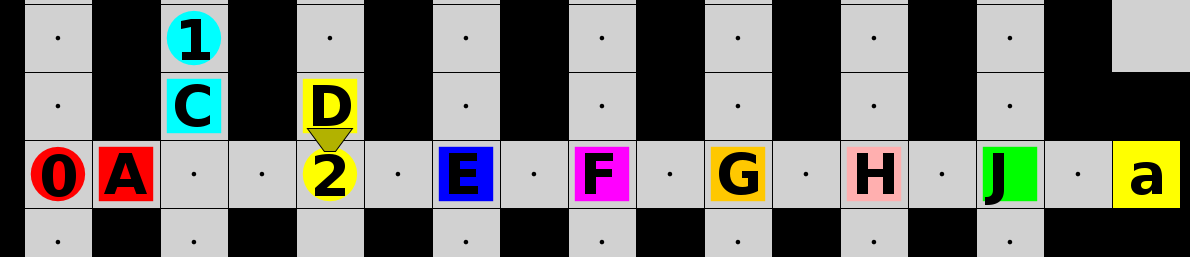
\includegraphics[width=.95\columnwidth]{graphics/planner_intuition.png}
  \caption{\label{fig:intuition example}The red agent \textbf{0} must move box \textbf{A} to the goal \textbf{a}.}
\end{figure}

However, the yellow agent \textbf{2} is now itself in the way of the path.
The planner thus informs that agent to move out of the desired path.
This moving of boxes/agents out of the way of the desired plan will continue until no more obstacles are in the way.
Then the red agent \textbf{0} will move the red box \textbf{A} to the goal.

\subsection{Goal Prioritisation Technique}
\label{methods:goal_ordering}

In order to explain how the functionality of our prioritisation works, we will break it down into three separate steps. For all the three steps we use an example set of goal cells, which are all only accessible form a single entrance. 

% Example of cells 
\begin{figure}[h!]
  \centering
  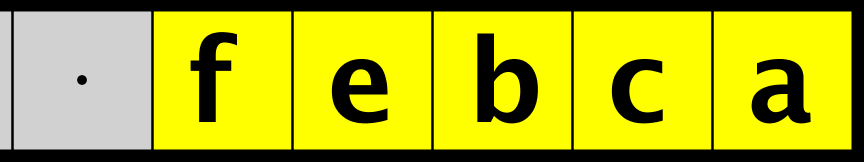
\includegraphics[width=.5\columnwidth]{graphics/ie_level.png}
  \caption{\label{fig:sample}Goal set with single entrance.}
\end{figure}

For the example in \cref{fig:sample} the optimal ordering would be to fulfil the goals in the following order: \textbf{a, c, b, e, f}, respectively.
To accomplish this, our algorithm provides an ordering score to each goal. 

\subsubsection{Evaluating Each Goals Neighbouring Cells}

Firstly, the algorithm evaluates each goal's eight neighbouring cells (including the diagonal neighbours). 
For every neighbouring goal-cell, the score of the goal that is being prioritised is incremented by 1.
For every free neighbour cell, the score is incremented by 2. 
The checking of neighbouring cells is illustrated with a grid in \cref{fig:grid1}. 
The middle cell is the one currently being checked, while the green represents a neighbour goal. 
A red cell represents an unreachable position (either a wall or out of bounds).

% Example of scoring 
\begin{figure}[ht!]
  \centering
  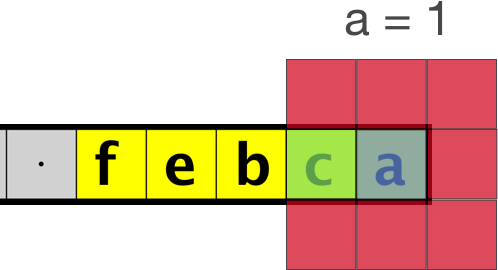
\includegraphics[width=.5\columnwidth]{graphics/goal_pri_1.png}
  \caption{\label{fig:grid1}Neighbour checking of goal \textbf{a}.}
\end{figure}

The goal \textbf{a} is given a start score of 1. 
Goal \textbf{f} and \textbf{b} are given scores of respectively 3 and 2 as can be seen in \cref{fig:grid2}. 
A blue cell in the grid represents a free neighbour, while a green cell represents a neighbouring goal.
The remaining goals not shown in the figures are all given a score of 2. 

% Example of scoring 
\begin{figure}[h!]
  \centering
  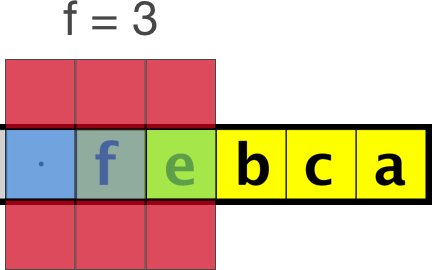
\includegraphics[width=.5\columnwidth]{graphics/goal_pri_3.png}
  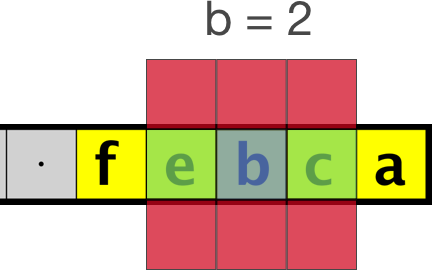
\includegraphics[width=.5\columnwidth]{graphics/goal_pri_2.png}
  \caption{\label{fig:grid2}Neighbour checking of goals \textbf{f} and \textbf{b}.}
\end{figure}

\subsubsection{Forcing an Order }
Secondly, after scoring the goals according to their neighbours, the algorithm creates an $n \times n$ size matrix, where $n$ is the number of goals. 
Each column of the matrix will represent a goal cell and the first row holds the ordering scores that were computed in the first step. 

\begin{table}[h!]
  \caption{\label{tab:example_matrix}\centering Example level - Ordering matrix \break Incomplete (left) \& Complete (right)}
	\begin{minipage}{.5\linewidth}
    \centering
    \begin{tabular}{@{}lllll@{}}
		\toprule
		\textbf{f} & \textbf{e} & \textbf{b} & \textbf{c} & \textbf{a} \\ \midrule
		3          & 2          & 2          & 2          & 1          \\ 
		-          & -          & -          & -          & -          \\ 
		-          & -          & -          & -          & -          \\ 
		-          & -          & -          & -          & -          \\ 
		-          & -          & -          & -          & -          \\ \bottomrule
		\end{tabular}
  \end{minipage}%
  \begin{minipage}{.5\linewidth}
    \centering
    \begin{tabular}{@{}lllll@{}}
		\toprule
		\textbf{f} & \textbf{e} & \textbf{b} & \textbf{c} & \textbf{a} \\ \midrule
		3          & 2          & 2          & 2          & 1          \\ 
		4          & 2          & 3          & 2          & 1          \\ 
		5          & 3          & 3          & 2          & 1          \\ 
		6          & 4          & 3          & 2          & 1          \\ \midrule
		\textbf{7} & \textbf{4} & \textbf{3} & \textbf{2} & \textbf{1} \\ \bottomrule
		\end{tabular}
  \end{minipage} 
\end{table}

The resulting matrix can be seen in \cref{tab:example_matrix} (left). 
From this matrix we see the first ordering scores being filled out while the rest remains to be computed. 
The computation of the remaining rows, is carried out by incrementing the scores iteratively. 
A goal's score is incremented if:

\begin{itemize} 
\item{The score is the maximum score of all score}
\item{The score is smaller than the previous and next score }
\item{The score is smaller than previous and equal to then next score}
\end{itemize} 

The idea is that we force an order on grouped goals so that we never have ambiguous priorities for neighbouring goals.
Thus, the client should never be in doubt of which goal to choose.

\subsubsection{Sorting the Goals}
Lastly, after the matrix has been filled as presented in \cref{tab:example_matrix} (right), the last row should contain the ordering of the goals.
These can then be used to order the goals in ascending order (from lowest to highest).
This steps responsibility is simply to order the goals, such that in our example case, the goals will be filled from \textbf{a} to \textbf{f}, respectively.
The performance benefits and pitfalls of this prioritisation algorithm, will be discussed in detail in \cref{subsec:disc_goal_ordering}.
\todo[inline]{remember to add this discussion section}
%
% In levels where goals are grouped independently of other goal groups, the algorithm will allow for some scores to be the same.
% This signals that some goals can be achieved in an arbitrary order without one having to be filled before the other.
% The last row of the matrix in \cref{tab:example_matrix} (right), is now used to order the goals.

\subsection{Representing a Level}
\label{sec:representing a level}

\subsubsection{Cell of a Level}

We represent levels as grids of cells, where each cell can hold a wall, goal, agent, or a box.
Otherwise it is a free cell.
Each cell is uniquely referenced with coordinates, that define the x and y coordinates w.r.t. the top left corner.
Thus, the first cell is referenced as $(0,0)$ and is in the top left corner of the level.

\subsubsection{The Grid}

A new grid object is instantiated with the level parsed from the server.
The grid instantiation process takes care of assigning default colors to uncolored objects.
The grid keeps track of the following; all object's positions (their cells) and colors, goals and their identifiers, the boxes and the agents.
It knows which color boxes an agent can move.
Furthermore, the grid representation must have the following functionality
%
\begin{itemize}
  \item for a given cell, return its neighbouring cells
  \item for a given cell, is it possible to perform a swapping move
  \item for all goals, compute their priority (see \cref{methods:goal_ordering})
  \item for every server response (with every action we send), update the grid so it is up-to-date
\end{itemize}
%
The neighbours of a cell may be defined to filter results w.r.t. some criterion.
Such a criterion could for instance be that we only want free cell (no agent or box at that cell).
This method is used for finding possible movement from a given cell.
Unlike in our goal prioritisation, where a cell has 8 neighbours, the diagonal cells are not considered neighbour cells here and thus a cell only has 4 neighbours.
%Moreover, a cell's neighbours are the cells below, above, right of, and left of it (not diagonal cells).

We define a swapping move as swapping the position of an agent and a box it is moving.
This could either be a pull-push combination or vice versa.
The idea is to check if a given cell has enough neighbours for a swap to be performed, i.e. the cell must have at least three neighbours (because then we at least have a \texttt{T}-cell-combination, where a swap is possible).

The client performs online planning, i.e. an entire complete plan is not computed before performing actions.
Because of this the client must keep track of all actions and if they succeed.
The server's response must be used to keep the level representation up-to-date.

\subsubsection{Movable Objects}

We define agents and boxes as movable objects.
They have a position (a cell), some color, and an identifier that uniquely defines them in the level.
Such an object can thus also be moved, which changes the position at which it is for that time step.

\subsubsection{Updating the Representation}

For every action sent to the server, we make sure to update the client's perception of the current environment.
Positions of agents and boxes are thus kept up-to-date while actions are performed.

\subsection{Constructing Paths and Searching}
\label{sec:constructing paths and searching}

Given a goal to achieve we split path finding into two parts; first find a box closest to the goal, second find the closest agent to move that box.
These two paths are then combined to form a complete path for movement (we explain the path finding in more detail later in this section).
The overall idea of our client is to iteratively remove obstacles from the combined path to reach the desired goal with the chosen box.
We customised the A* search algorithm~\cite{pathfinding2016redblobgames} to suite our needs for finding paths.

\subsubsection{Distance to Goal}

We used the cross product as a heuristic to prioritise movement wrt. cells and their distance to the goal cell.~\cite{pathfinding2016redblobgames}
We search for paths in a relaxed domain, where boxes and agents are not considered as blocking objects, but the cells in which they are have a higher movement penalty.
This is similar to the ignore preconditions heuristics, because we ignore that the cell must be free before movement is possible.
The client then handles the fact that some other object must be moved before the initial plan can be carried out.

\subsubsection{Movement Cost}

While searching for a path to a desired end position, four scenarios may occur; (1) the object can move freely in the given direction, (2) the object must move an obstacle to move in the given direction, (3) the object must receive help to move an obstacle, (4) another agent must be moved to move in the given direction.

These scenarios are associated with different costs, and they are as follows; cost of receiving help is 20, cost of moving an obstacle (without help) is 4, cost of asking an agent to move is 3, otherwise object can be moved freely and the cost is 1.
We wanted the movement of one agent to be as independent as possible from other agents.
For that reason we associated higher costs for receiving help from other agents, and if an agent can move around an obstacle it will prefer that over moving the object itself.

\subsubsection{Ignoring Heuristics}

In some scenarios an object must be moved from a desired path, because it is blocking the desired path.
For this we ignore the distance to the goal because we do not have a desired end position, we simply need to find the first free cell where the object can be moved to, which gets it out of the desired path.

\subsubsection{Structuring Paths and Converting to Actions}

Path movement is initially a list of coordinates dictating the movement of an object.
Thus, consecutive elements of the list comprise a single step in one direction.
The first element in the list gives the position of the object to be moved.
The grid can inform what object is at that position.
The path of cells is converted to a list of actions, which the server can interpret.

The list of coordinates also defines when an agent is to move a box.
This is defined as a list in the outer list, i.e. in this scenarios an element in the outer list is not a tuple but a nested list, e.g. \texttt{[(0,0),[(0,1),(1,1)],(0,1)]}.
The example will be interpreted to \texttt{[Push(E,S)]}, where the nested list defines the initial position of the box and the following movement.
The element after the inner list defines the end position of the agent that was involved in the moving action.

\subsection{Planning on the Fly}
\label{sec:planning on the fly}

We perform online planning, i.e. we do not create an entire complete plan before executing movement.
Given a constructed plan as described in \cref{sec:constructing paths and searching} the client, that plan may contain positions on which obstacles are in the way.
Given that obstacle the client will create a new sub-plan, which must be achieved before the original plan can continue.
This process may continue for many steps before all obstacles are moved for the original objects to be moved in the desired path.
Note however, that sub-plans of a sub-plan may also occur.

As mentioned in the previous section, each movement has an associated cost, and the agents are to be as independent as possible.
However, independence is sometimes not possible and thus the agents must aid one another.
The planner thus tries to create a sub-plan, where that plan's goal is to move the obstacle.
This is done in an iterative manner, where the planner checks if the current plan/sub-plan is conflict/obstacle free and thus returns a list of desired actions to the client, which then sends actions to the server.
The client monitors the execution of the agents in a similar fashion to action monitoring, but where we use the server's response to validate that our action was successful and from that update the representation of the level's state.

The planner is continuously called with new goals to be achieved until all goals are occupied by a corresponding box.
Note, that a plan is created and executed for a single agent at a time.


